\documentclass[letterpaper,12pt]{article}
\usepackage[margin=1in]{geometry}
\usepackage{graphicx}  % Include figure files
\usepackage{xcolor}  % Allow for a color text
\usepackage{amsmath}  % math fonts
\usepackage{amsfonts}  % math fonts
\usepackage{latexsym}  % math fonts
\usepackage{amssymb}  % math fonts
\usepackage{mathtools} % Give more control of how equations are displayed
\usepackage{appendix} % Lets you create an appendix
\usepackage[numbered]{matlab-prettifier} % Let's me import MATLAB code in a nice format
\usepackage{indentfirst} % This indents the first paragraph. By default latex won't do it.
\usepackage{subfigure}

\setlength{\parskip}{1em} % This skips a line when making new paragraphs
\newtagform{show_eq}{(Eq.\ }{)}  % how the equation numbers are displayed
\usetagform{show_eq} % this goes with the \newtagform

\begin{document}

% ================================== Title Page ==========================================
\begin{titlepage}
 \begin{center}
 \vspace*{1in}
{\Huge LAB 7}\\
    \bigskip
    by\\
    \bigskip
    {\Large Kevin Moran} \\
    \bigskip
    Lab Partner : Cade Hermeston\\
    Date of Experiment : Thursday, October 29th, 2020

    \bigskip\bigskip\bigskip
    University of Southern California\\
    Aerospace and Mechanical Engineering Department\\
    AME 341A : Mechoptronics
 \end{center}
\end{titlepage}
% ----------------------- Abstract ------------------------------------
\begin{abstract}
    
\end{abstract}

% ------------------------- Introduction ----------------------------------
\section{Introduction}

% ---------------------------- M & M --------------------------------------- 
\section{Methods and Materials}

% ---------------------------- Results -------------------------------------
\section{Results}

% :::::::::::::::::: Sine and Square Wave Subsection ::::::::::::::::::
\subsection{Sine and Square Wave}

talk about the results that we got during the first part of the experiment. The conditions, setup, ect.
\begin{figure}[hbt!]
\centering
\subfigure[Sine Wave]{
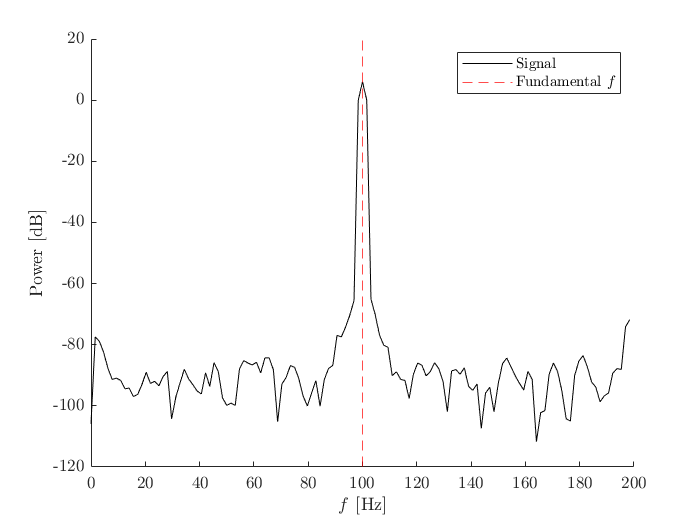
\includegraphics[width=.4\linewidth]{sin.png}}
\quad
\subfigure[Square Wave]{
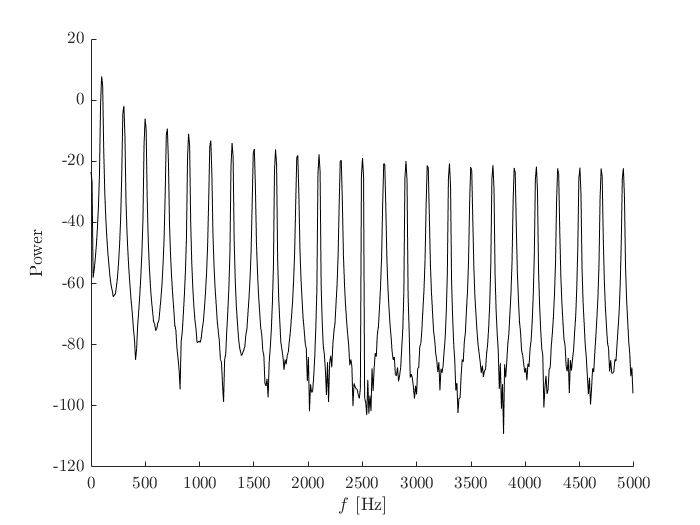
\includegraphics[width=.4\linewidth]{square.png}}
\caption{Sine and square waves with $V_{rms}$ of 2V at 100Hz shown in the frequency domain}
\end{figure}

% :::::::::::::::::: Aliasing Subsection ::::::::::::::::::
\subsection{Aliasing a Signal}
Explain how we can tell from our nyquin frequency how we know the values are being aliased

\begin{figure}[h!]
\centering
\subfigure[$f_s$ = 10 kHz]{
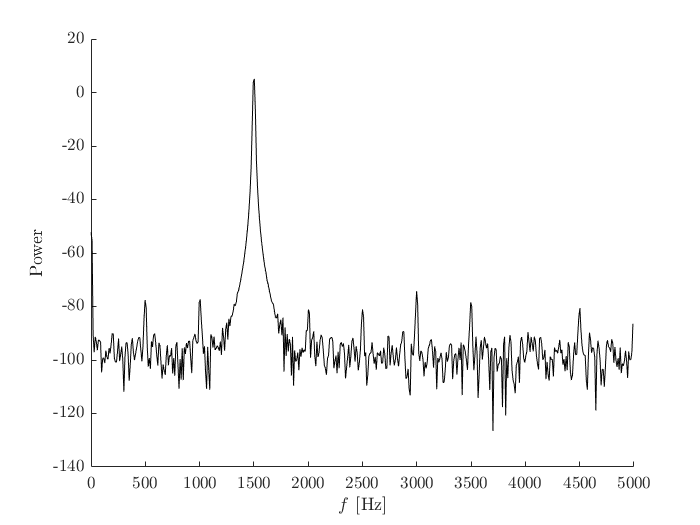
\includegraphics[width=.4\linewidth]{sin10000.png}}
\quad
\subfigure[$f_s$ = 2.5 kHz]{
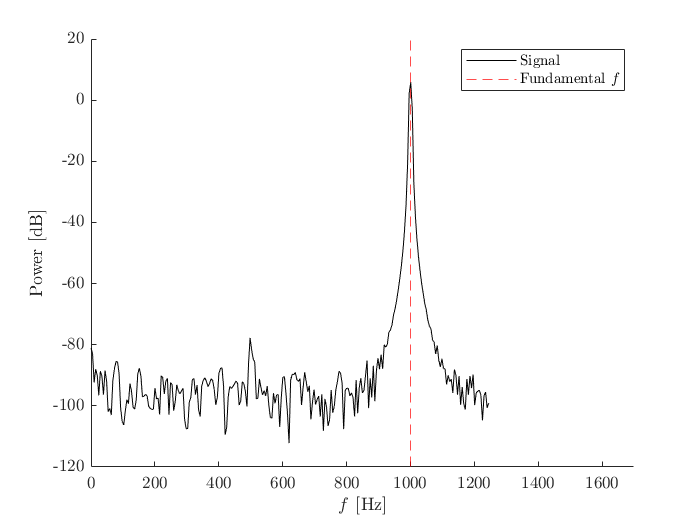
\includegraphics[width=.4\linewidth]{sine2500.png}}
\caption{Sine and square waves with $V_{rms}$ of 2V at 100Hz shown in the frequency domain}
\end{figure}

the images in the time domain

\begin{figure}[h!]
\centering
\subfigure[$f_s\ > \ f$]{
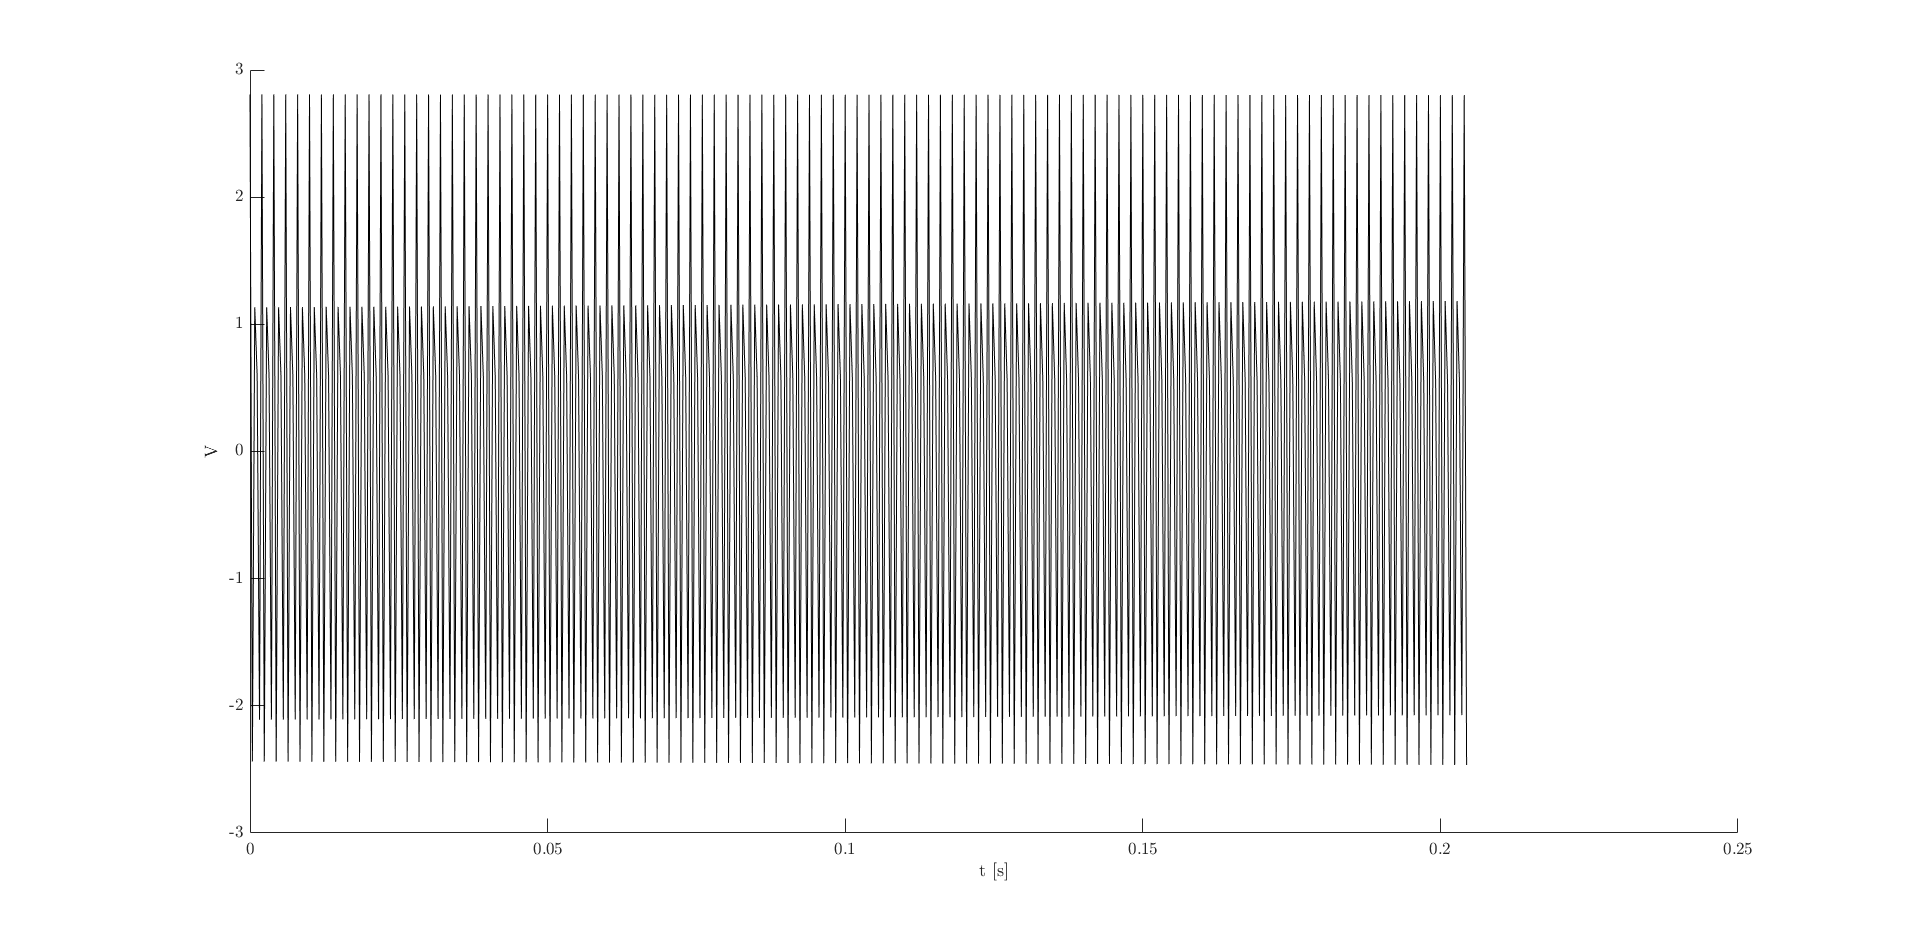
\includegraphics[width=.4\linewidth]{sineTime2500.png}}
\quad
\subfigure[$f_s\ = \ f$]{
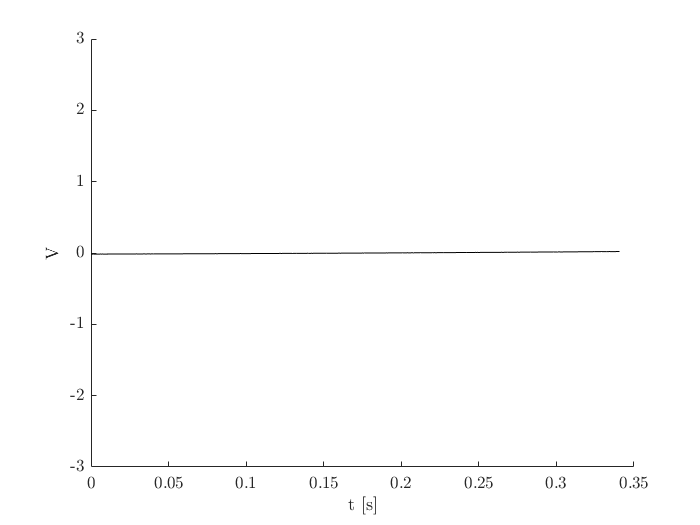
\includegraphics[width=.4\linewidth]{sineTime1500.png}}
\subfigure[$f_s\ < \ f$]{
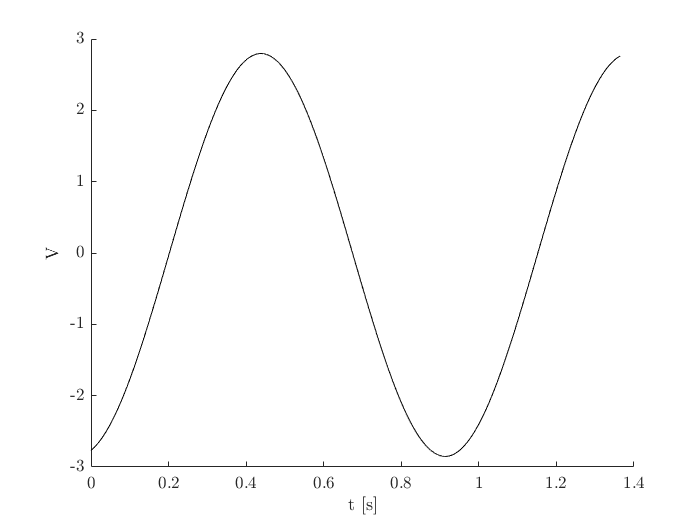
\includegraphics[width = .5\linewidth]{sineTime1501.png}}
\caption{Sine and square waves with $V_{rms}$ of 2V at 100Hz shown in the frequency domain}
\end{figure}





% :::::::::::::::::: Mystery Wave Subsection ::::::::::::::::::
\subsection{Analysis of Unknown Signal}
This is the part where we can explain what we measured in lab BUT DON'T MENTION ANYTHING ABOUT HOW WE FIGURED IT OUT YET!

\begin{figure}[h!]
    \centering
    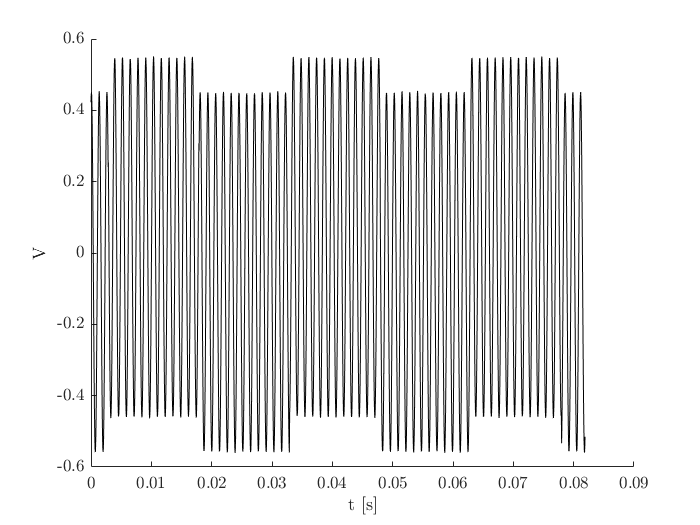
\includegraphics[scale=.7 ]{mysteryTime.png}
    \caption{Time trace of unknown signal}
    \label{UnknownTime}
\end{figure}

\begin{figure}[h!]
\centering
\subfigure[$f_s$ = 1 kHz]{
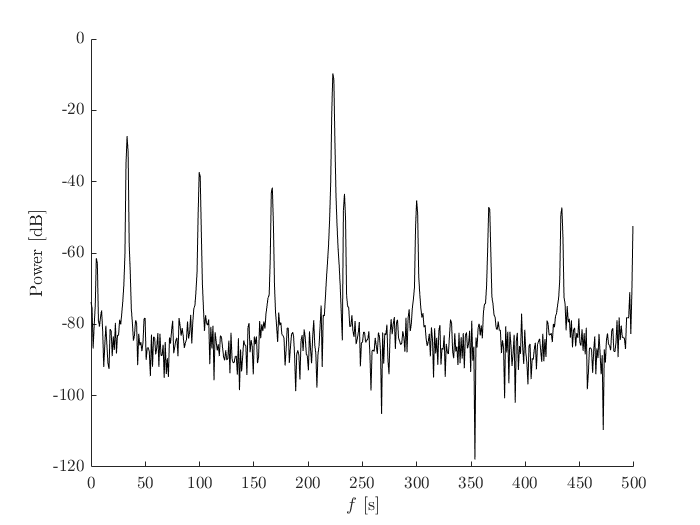
\includegraphics[width=.4\linewidth]{mystery1000.png}}
\quad
\subfigure[$f_s$ = 2 kHz]{
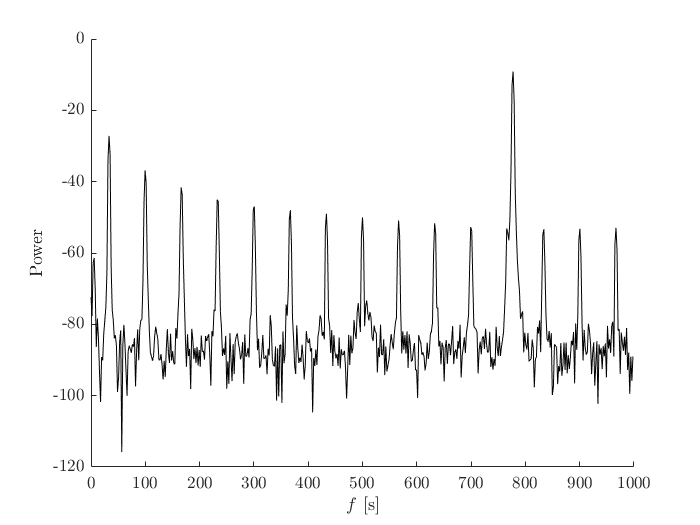
\includegraphics[width=.4\linewidth]{mystery2000.png}}
\caption{Sine and square waves with $V_{rms}$ of 2V at 100Hz shown in the frequency domain}
\end{figure}


% ---------------------------- Discussion -------------------------------
\section{Discussion}

% ---------------------------- Conclusion -------------------------------------
\section{Conclusion}




\end{document}